\section{Performance}
\label{Sec:Perf}

In order to increase the performance, and, even more importantly, the perceived performance and responsiveness, of our application, we implemented the techniques discussed below.
While the assignment suggests applying these to the MIP renderer, we implemented these generally, which means they work for all the methods in our raycaster (with the exception of the slicer, which ignores resolution).

\subsection{Resolution}
The first and most obvious technique we apply is changing the resolution of the image.
By calculating the image on a lower resolution, we can reduce the calculation time by a significant factor.

Changing the resolution is implemented simply by dividing the virtual image size by a certain factor, and taking samples as if we were actually rendering for this image size.

However, as one might expect, while this technique speeds up the calculation, it also greatly reduces the quality of the image.
The results of rendering the \texttt{orange.fld} data set (using MIP) with different resolution factors can be seen in Figure~\ref{fig:perf:comp}.

\begin{figure}[H]
	\centering
	\begin{subfigure}[t]{0.45\textwidth}
		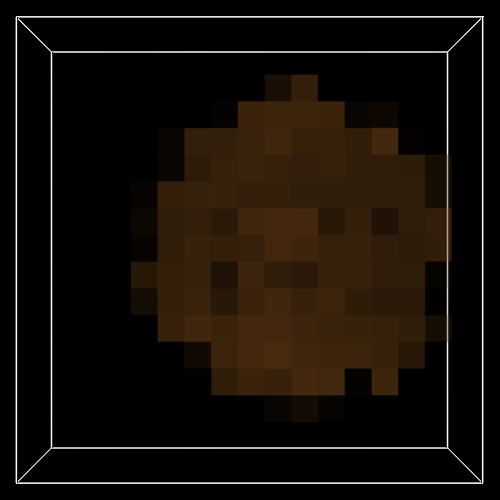
\includegraphics[width=\textwidth]{fig_perf_comp_16}
		\caption{Rendering at factor 16}
	\end{subfigure}
	~%
	\begin{subfigure}[t]{0.45\textwidth}
		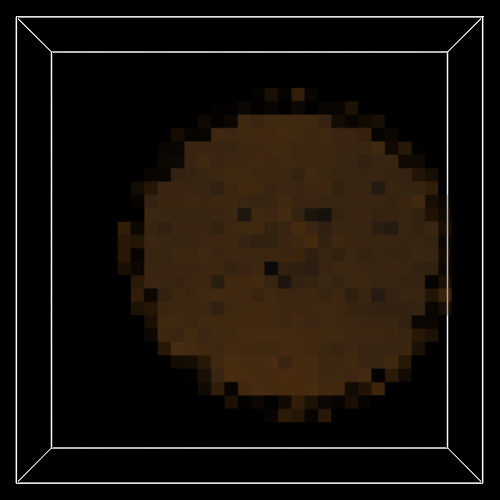
\includegraphics[width=\textwidth]{fig_perf_comp_8}
		\caption{Rendering at factor 8}
	\end{subfigure}
	
	\begin{subfigure}[t]{0.45\textwidth}
		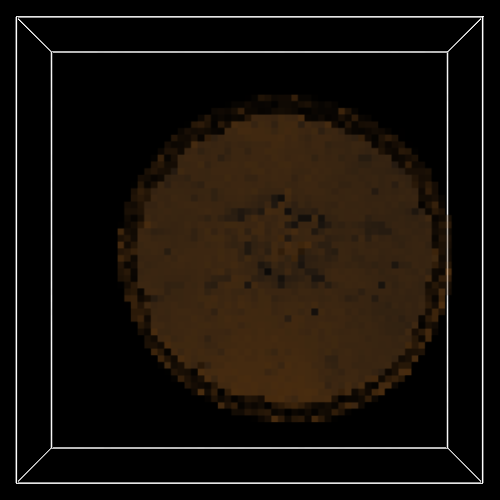
\includegraphics[width=\textwidth]{fig_perf_comp_4}
		\caption{Rendering at factor 4}
	\end{subfigure}
	~%
	\begin{subfigure}[t]{0.45\textwidth}
		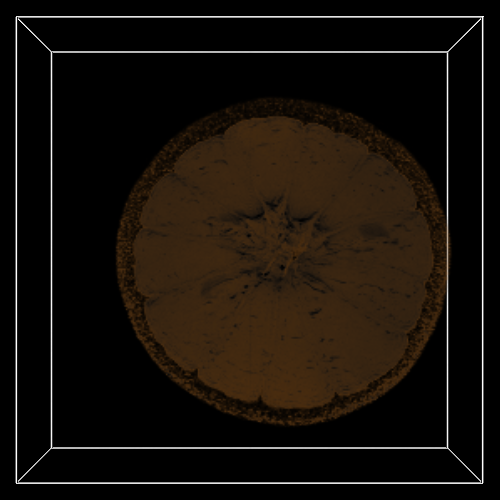
\includegraphics[width=\textwidth]{fig_perf_comp_1}
		\caption{Rendering at factor 1 (no resolution change)}
		\label{fig:perf:comp:1}
	\end{subfigure}
	
	\caption{A comparison of rendering \texttt{orange.fld} on different resolution factors}
	\label{fig:perf:comp}
\end{figure}

\subsection{Adaptive resolution scaling}
An important annoyance while working with the VolVis program was the fact that it takes too long for settings to apply.
It is hard to easily rotate the model or tweak the transfer function to get a better result when rendering each step takes a long time.
To combat this, we started rendering at lower resolutions.

However, these lower resolutions are not satisfactory when the goal is to really inspect a model.

Because of this, we adopted adaptive resolution scaling.
This means that when the user actively interacts with the application (by rotating the model, changing the field of view or modifying parameters) the renderer will immediately fall back to a resolution at which it can render fast.
Thus, the end user can immediately see the result of their action, albeit at a lower resolution.
When the user does not touch the controls for a while, the application will scale down the resolution factor bit by bit, thereby increasing the quality of the rendering.
After some testing, we determined that a good bound to stop increasing the quality is when the calculation for a rendering takes about 500ms.
After this, the calculations become too heavy to do under normal circumstances.

This however means that on most hardware, the user will not see the best available rendering.
To combat this, we created a 'force quality' mode that effectively ignores the renderer's cues to scale down the quality.
When the 'force quality' mode is turned on (controlled by a checkbox in the user interface), the application will continue to ramp up the quality until a resolution scaling factor of 1 is reached, as shown in Figure~\ref{fig:perf:comp:1}.

Effectively, this technique allows for fast and responsive tweaking of parameters and position in order to design a good interpretation of the data, while also making it easy to render the resulting image at a high quality.

\subsection{Exporting images}
Another technique that allows users to quickly get to the right parameters but with a high quality image is exporting.

When a user chooses to export, a new background render will be started with the current parameters, but with the highest resolution possible.
The application can save to a PNG file.
Note that transparency created by the transfer function will be maintained in the exported image file, making this a very useful tool for re-using generated images in some way (for example reports or web pages).

An example export created by our application is given in Figure~\ref{fig:perf:export}.

\begin{figure}[H]
	\centering
	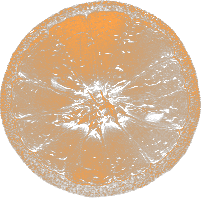
\includegraphics[width=0.5\textwidth]{fig_perf_export}
	\caption{Exported render of \texttt{orange.fld}}
	\label{fig:perf:export}
\end{figure}

\subsection{Background rendering}
\label{Sec:Perf:Background}
While inspecting the given project skeleton, we noticed that the calculation of the image is done during OpenGL rendering.
This means that the calculated image is always 'up to date' with the set parameters, but it is not really nessecary to calculate the image at that time.

To further improve the responsiveness of the application, we moved the image calculation to a background thread.
The last available calculated image is stored in the renderer.
When the renderer visualizes the image, it will use the last available known image, and then start the calculation of a new image in the background thread.
While this means that an image can be 'one frame' behind the set parameters, we have found that this makes no noticeable difference for the end user.

Doing the calculations in the background of course means that the user interface will not 'freeze' when heavy calculations are made.

To make sure the application does not use more resources than nessecary, the renderer will reject new requests for calculations while a calculation is running.
However, when the new request is due to some changed parameter, the renderer will cancel the running calculation (which is now useless) and start a new one.
At the same time, changes to such parameters (and mouse actions) will lead to an immediate drop in quality.

This leads to an ever better responsiveness (and thus, user experience), since the program will respond to changes very quickly.

However, when a user is interacting heavily with a visualization through rotations, running calculations in the foreground thread can feel a bit more 'snappy'.
Because of this, we built in an option to disable background calculations.
When background calculation is off, the program will still spawn new threads to run calculations, but it will wait on the result of the computation before leaving the OpenGL render routine.
